
\documentclass[12pt,a4paper]{report}
\usepackage[english]{babel}
\usepackage[T1]{fontenc}
\usepackage{times}
\usepackage{amsmath}
\usepackage{amsfonts}
\usepackage{amssymb}
\usepackage{textcomp}
\usepackage{gensymb}
\usepackage{hyperref}
\usepackage{graphicx}
\usepackage{setspace}
\usepackage[version=4]{mhchem}
\usepackage{caption}
\usepackage{subcaption}
\usepackage{longtable}
\usepackage[dvipsnames]{xcolor}
\usepackage{tikz}
\usepackage{wrapfig}
\usepackage[left=2cm,right=2cm,top=2cm,bottom=2cm]{geometry}
\makeatletter
\newcommand\footnoteref[1]{\protected@xdef\@thefnmark{\ref{#1}}\@footnotemark}
\makeatother
\graphicspath{{IMAGE/}}

    \makeatletter
\newcommand{\AlignFootnote}[1]{%
  \ifmeasuring@
  \else
    \iffirstchoice@
      \footnote{#1}%
    \fi
  \fi}
\makeatother



\begin{document}

\begin{titlepage}

\centering

\includegraphics[scale=0.25]{logo_ulg.png}%

\begin{center}\bfseries\huge
\vspace*{1cm}
Modeling and design of electromagnetic systems
\end{center}

\begin{center}\normalsize
Professor: C. Geuzaine\\
\end{center}

\vspace*{\stretch{1}}
\hrulefill
\begin{center}\bfseries\Huge
Homework 3 
\end{center}

\hrulefill
\vspace*{1cm}
\begin{center}\bfseries\Large
Sour Nassim, Heylen Martin
\end{center}

\begin{center}\bfseries\large

Master in electromechanical engineering\\ Bloc 2 \\
University of Liège \\
Academic year: 2019-2020
\end{center}
\vspace*{\stretch{2}}
\begin{flushright}

\end{flushright} 

\end{titlepage}
\setstretch{1.5}
\chapter{Introduction}
\quad\, This project is dedicated to the study of three-phase transformers. Those components are essential in the electrical network to switch from one voltage value to an other, or to reroute some part of the power to equaly distribute the power flow through the different branches of the network. Figure \ref{fig:real_transformer} shows the picture of a typical three-phase transformer.

\begin{figure}[h]
    \centering
    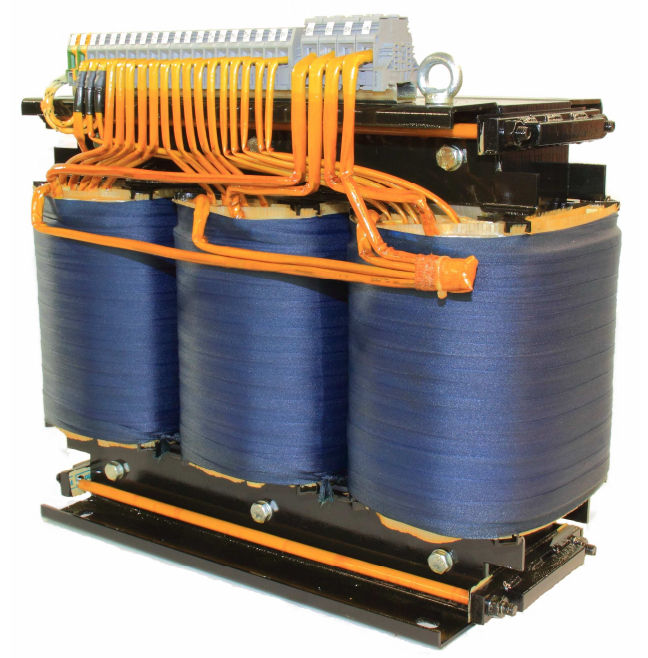
\includegraphics[width=0.4\textwidth]{real_transfo.jpg}
    \caption{Example of real three-phase transformer}
    \label{fig:real_transformer}
\end{figure}
\newpage
\chapter{Upstream analysis}
In this chapter will be introduced all the required elements to conduct the analysis of the studied three-phase transformers. Here, two transformers, respectively named \textbf{A} and \textbf{B}), of two different sizes will be considered in this report. The first one is a small transformer that makes the voltage going from 2.4 kV to 240 V for a nominal apparent power of 200 kVA. Let's define the transformer ratio $N$ as being the ratio between the secondary and the primary terminal voltage values. For this transformer, the transformer ratio is equal to 

\begin{equation}
\setstretch{1}
    N_A = \frac{240}{2400}\cdot 100 = 10\%
\end{equation}

The second transformer is bigger since it works between the 60 kV and 2.4 kV (leading to a transformer ratio of 4\%). The nominal apparent power of this transformer is equal to 20,000 KV.

These characteristics supposed that the network is at 50 Hz. Those are summarized in Table \ref{tab:characteristics_transfo}.

\begin{table}[h]
    \centering
\begin{tabular}{l|ll}
Transformer type   & \textbf{A}             & \textbf{B} \\ \hline
Input voltage [V]  & 2400                   & 60000      \\
Output voltage [V] & 240                    & 2400       \\
Output power [kVA] & 200                    & 20000      \\
Frequency [Hz]     & \multicolumn{1}{c}{50} & 50        
\end{tabular}
    \caption{Specifications of the two three-phase transformers}
    \label{tab:characteristics_transfo}
\end{table}

In the statement of the project, there is no information about if the given voltages are phase-to-phase or phase-to-neutral. Also, it is not indicated if those are peak or RMS values. Therefore, it will be assumed that the specified voltage are phase-to-phase RMS voltage.

Therefore, the nominal apparent power $S_N$ is defined as follows

\begin{equation}
\setstretch{1}
    S_N = \sqrt{3}\cdot U_N\cdot I_N
\end{equation}

where $U_N$ is the nominal phase-to-phase voltage (RMS value) and $I_N$ is the nominal current (RMS value). Note that the link between the RMS value and its equivalent peak value can be found by using

\begin{equation}
    Peak_{value} = RMS_{value} \cdot \sqrt{2}
\end{equation}


\section{Type of three-phase transformer}
\quad\, When considering a three phase transformer, several configurations regarding to the construction of the core.

The first type of transformer consists in connecting three single-phase transformers together. This configuration is suitable for transformers of large nominal power. Also, "in case of failure of one of the transformers, only that transformer is replaced"\footnote{\url{http://www.montefiore.ulg.ac.be/~vct/elec0014/transp-t.pdf}}. It is also easier to carry.

The second type of three-phase transformers are ones for which the core is shared for the three phases. Thus, this implies that the phases are coupled together.

Also, the "volume of this common core is smaller than three times the volume of a single core".

In this project, the magnetic material used for the core is soft iron for which the saturation induction is around 2T. Also, since it has been said that three individuals core were more suitable for big transformers, transformer \textbf{B} will be design in this way.

\section{Choice of the three-phase transformer connections}
\quad\, Once the core(s) is(are) designed, the second step is to make a decision regarding to the type of connection of the different phases. Basically, considering one side of the transformer, the winding can either be connected in \textcolor{red}{star} or \textcolor{green}{delta}.
\subsection{Star connection}
\quad\, The star connection consists in connecting each of three phases to a common nodes which is usually grounded. The star connection is depicted on Figure \ref{fig:star}.
\begin{figure}[h]
    \centering
    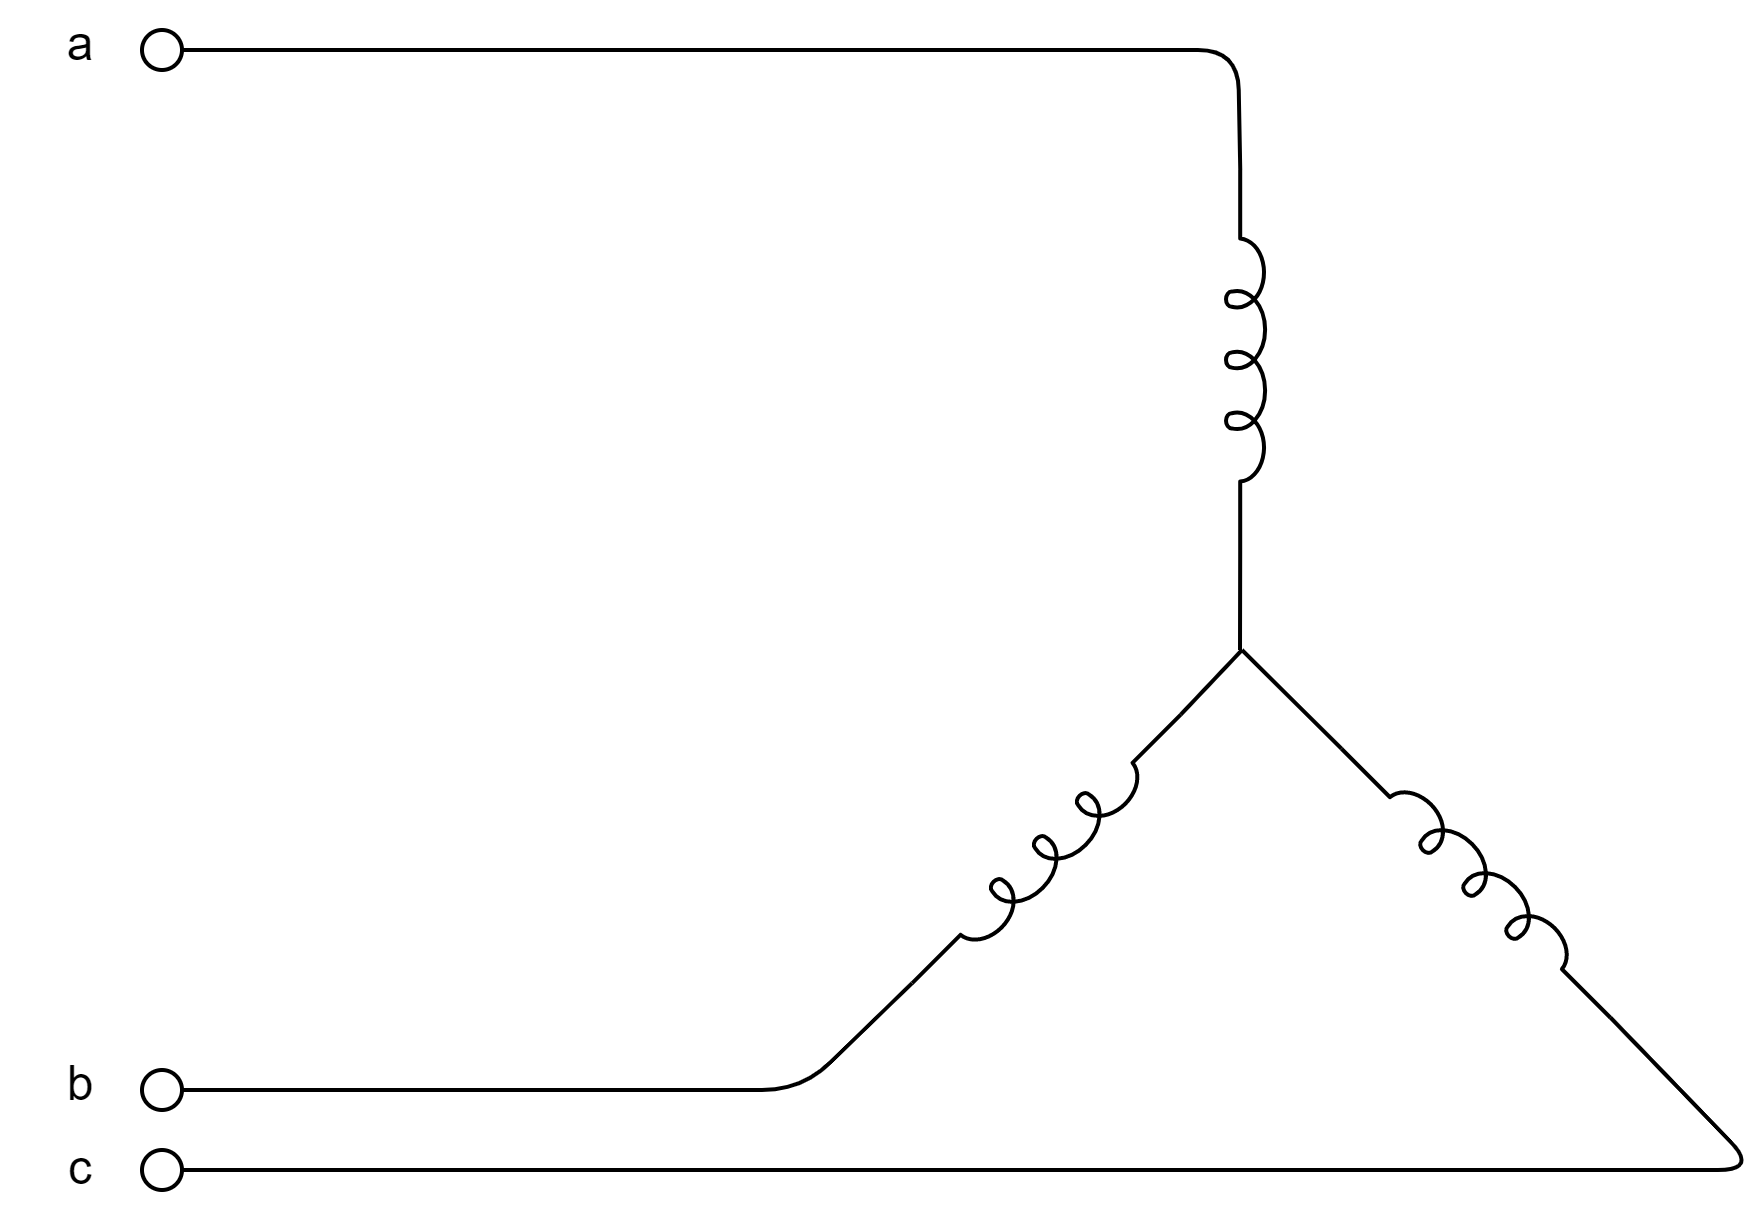
\includegraphics[width=0.5\textwidth]{Star.png}
    \caption{Three phase device - Star connection}
    \label{fig:star}
\end{figure}

The advantages of this type of connection are multiple. First, in case of a fault, the really high current generated due to this fault can be evacuated through this grounding connecting. Also, the star connection are usually used for the high voltage side of the transformer because it allows to cut by $\sqrt{3}$ the voltage in each phase of the transformer.

\subsection{Delta connection}
The second type of connection of the three phases are delta connection. Here, the each extremities of a winding are connected to the two others phases, creating a closed loop. The delta configuration is illustrated on Figure \ref{fig:delta}.

\begin{figure}[h]
    \centering
    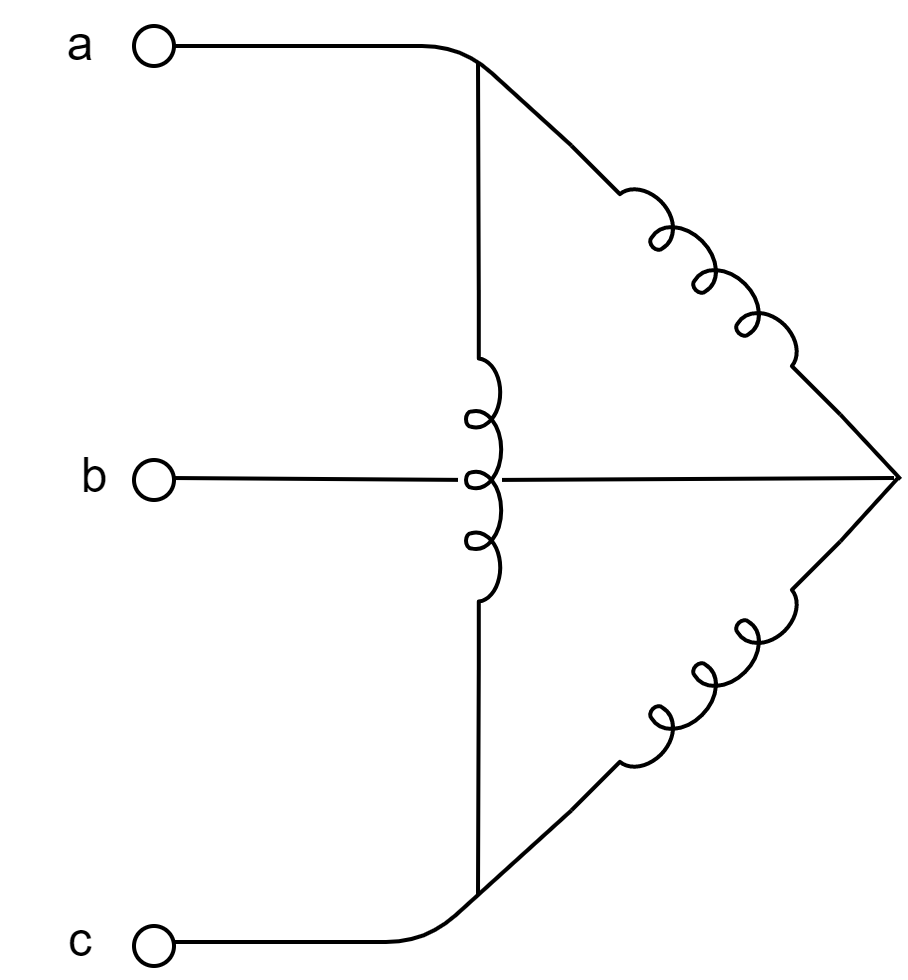
\includegraphics[width=0.5\textwidth]{Delta.png}
    \caption{Three phase device - Star connection}
    \label{fig:delta}
\end{figure}

Considering a current of intensity I injected in each lines \textit{a}, \textit{b}, and \textit{c}, it can be demonstrated that the current flowing through the branches of the transformer is $\sqrt{3}$ smaller.

Usually, when considering a three-phase transformer, the connections at the low voltage side follow the delta type to minimize the current flowing in the winding of the transformer.
\newpage
\subsection{Transformer - Possible mountings}
\quad\, The two previous subsections described the two possible type of connection of a three-phase device. Considering a transformer, the primary and secondary sides can be both considered as two three-phase devices. Thus, there are four possible mountings for the transformer.

\begin{itemize}
    \item Star-Star: The primary and secondary sides are both connected in star. This configuration, that can be met for high-voltage (HV) phase-shifting transformer, is depicted in Figure \ref{fig:star-star transformer}. 
    \begin{figure}[h]
    \centering
    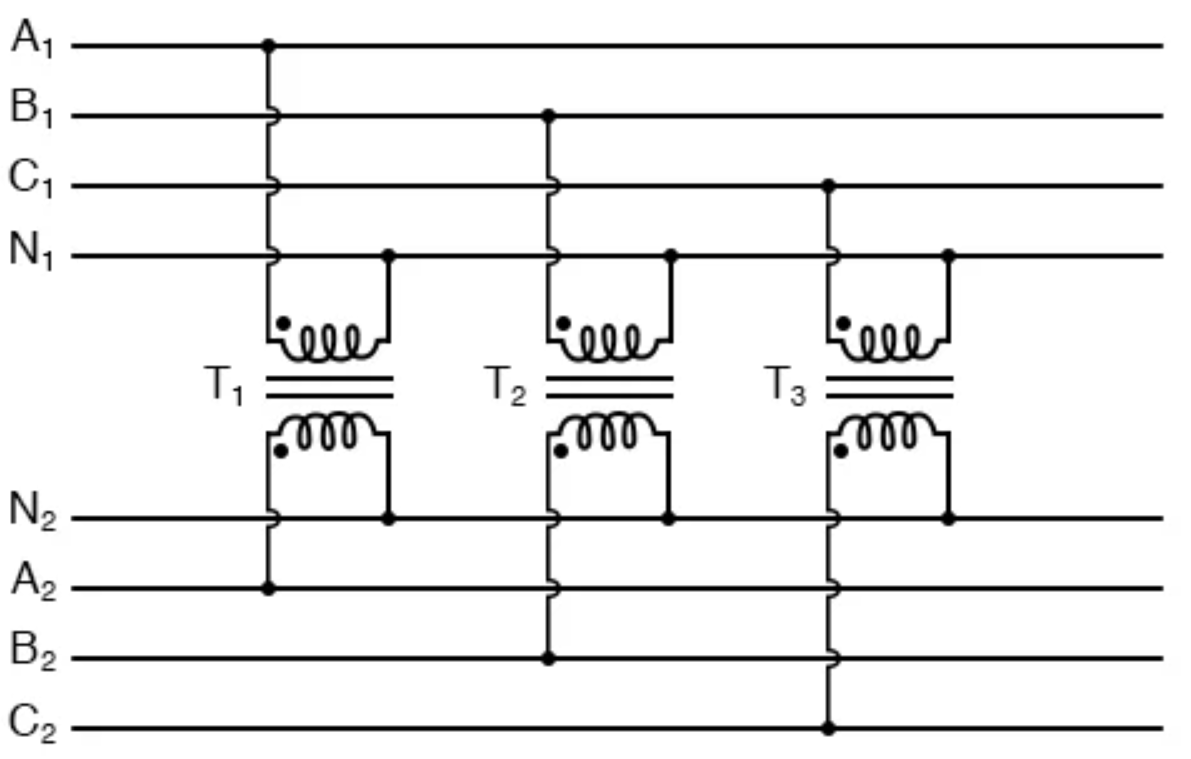
\includegraphics[width=0.6\textwidth]{y-y.PNG}
    \caption{Star-Star three-phase transformer}
    \label{fig:star-star transformer}
    \end{figure}
    
    \item Delta-Delta: The primary and secondary sides are both connected in delta. This configuration, that can be met for low-voltage (LV) phase-shifting transformer, is depicted in Figure \ref{fig:delta-delta transformer}. 
    \begin{figure}[h]
    \centering
    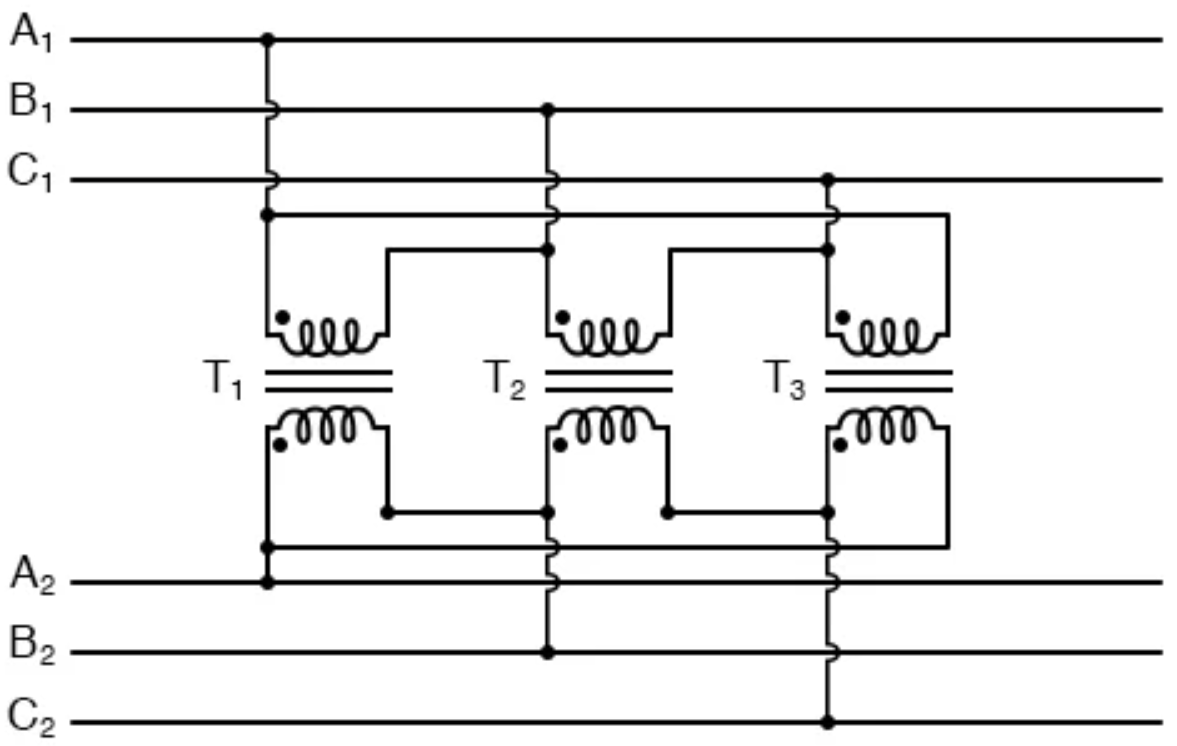
\includegraphics[width=0.6\textwidth]{delta-delta.PNG}
    \caption{Delta-Delta three-phase transformer}
    \label{fig:delta-delta transformer}
    \end{figure}
\end{itemize}
\newpage
\begin{itemize}
    \item Delta-Star: The primary side is wired in delta while the secondary side follows the star configuration. Delta-Star transformers are often used for step-up transformer because high current will flows in the primary side. Figure \ref{fig:delta-star transformer} depicts such configuration. 
    \begin{figure}[h]
    \centering
    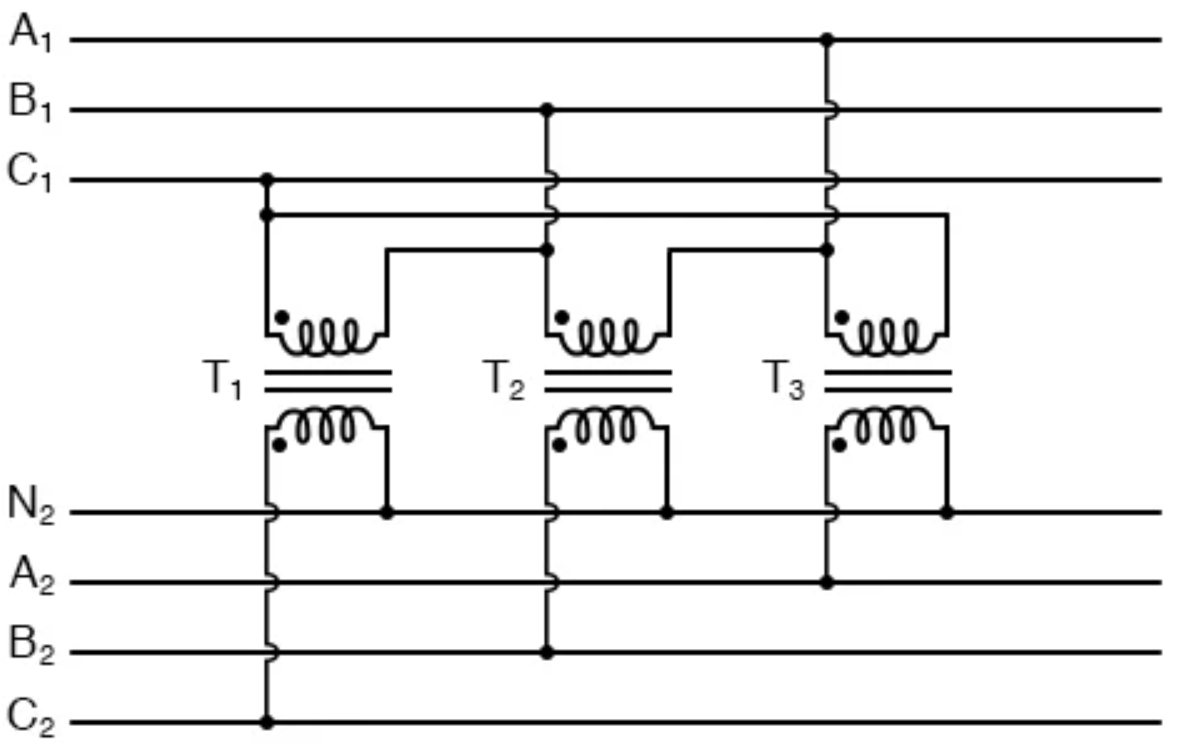
\includegraphics[width=0.6\textwidth]{delta-y.PNG}
    \caption{Delta-Star three-phase transformer}
    \label{fig:delta-star transformer}
    \end{figure}
    
    \item Star-Delta: The primary side is wired in star while the secondary side follows the delta configuration. Star-Delta transformers are often used for step-down transformer because high current will flows in the secondary side. Figure \ref{fig:star-delta transformer} depicts such configuration.  
    \begin{figure}[h]
    \centering
    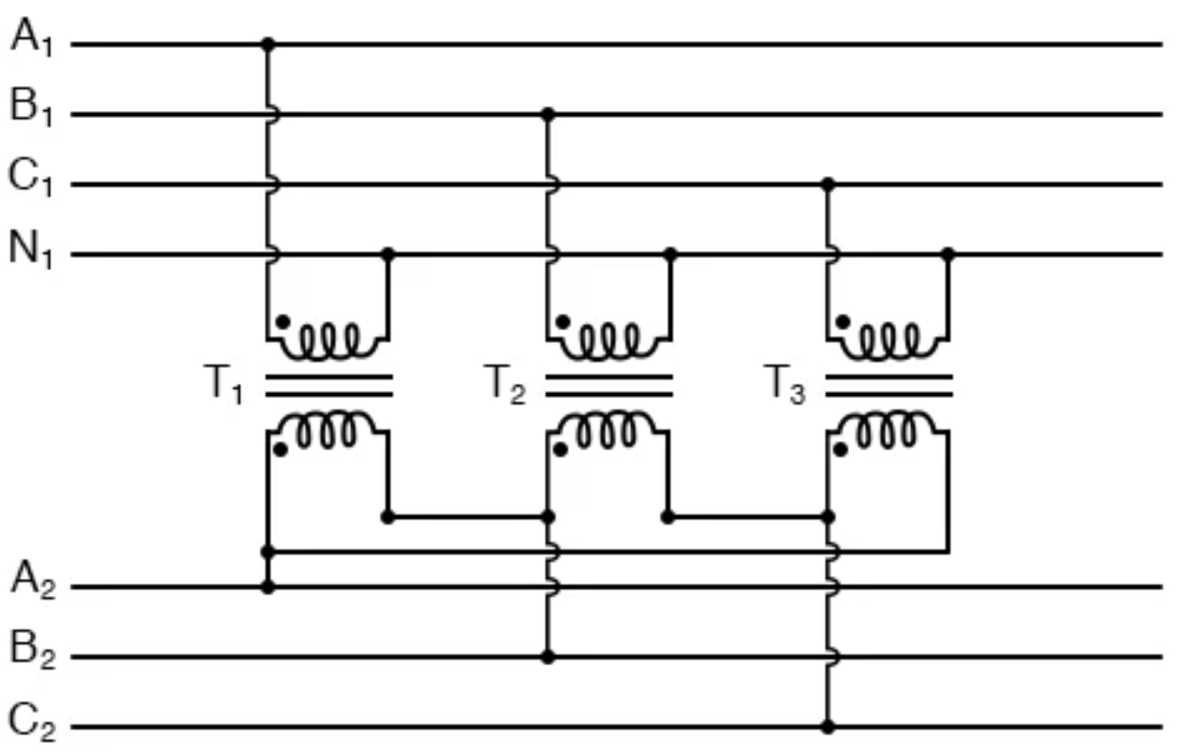
\includegraphics[width=0.6\textwidth]{y-delta.PNG}
    \caption{Star-Delta three-phase transformer}
    \label{fig:star-delta transformer}
    \end{figure}
\end{itemize}

Considering that the two studied transformers for this project are step-down transformers, the retain wiring configuration is the Star-Delta configuration.

\section{Nominal values}
\quad\, In the beginning of the chapter, the characteristics of the two transformers have been established. The nominal apparent power $S_N$ have been defined as being

\begin{equation}
\setstretch{1}
    S_N = \sqrt{3}\cdot U_{N,1}\cdot I_{N,1} = \sqrt{3}\cdot U_{N,2}\cdot I_{N,2}
\end{equation}

Therefore, considering the two transformers \textbf{A} and \textbf{B}, the nominal current that has to be sustained by the conductors can easily be obtained by replacing the nominal voltage and apparent power value by the ones in Table \ref{tab:characteristics_transfo}. The results of the calculations are included in Table \ref{tab:currents}.

\begin{table}[h]
    \centering
    \begin{tabular}{l|ll}
    Transformer                                  & \textbf{A} & \textbf{B} \\ \hline
    Nominal RMS current [A] - Primary side   & 48.11                       & 192.45                      \\
    Nominal RMS current [A] - Secondary side & 481.12                      & 4811.25                    
    \end{tabular}
    \caption{Primary and secondary currents of the two design}
    \label{tab:currents}
\end{table}


\section{Diameter of the windings}\label{diameter}
\quad\, As it has been mentioned in the previous section, the conductors has to be designed such that the specified nominal currents can be sustained an infinite amount of time without causing damages.

It has been established that the maximum current density $J_{copper,max}$ of the copper is equal to 2 A/mm$^2$. Thus, by applying the formulae \ref{eq:Imax}, the cross-section of the conductors can be computed.

 \begin{equation}
 \setstretch{1}
    I_{1,2} =  J \cdot A_{1,2}\label{eq:Imax}
\end{equation}

Where $I_{1}=I_{N,1}$ and $I_{2}=\frac{I_{N,2}}{\sqrt{3}}$ since the current in each winding is $\sqrt{3}$ smaller than the current flowing through the lines.

Once the cross-section computed, the radius of the winding can be deduced. The Table \ref{tab:windings_A} includes the obtained results.
\begin{table}[h]
\centering
\begin{tabular}{l|llll}
Transformer             & \multicolumn{2}{c}{\textbf{A}} & \multicolumn{2}{c}{\textbf{B}} \\ \hline
Side                    & Primary       & Secondary       & Primary       & Secondary      \\
Nominal RMS current [A] & 48.11         & 481.12          & 192.45        & 4811.25        \\
Area [mm$^2$]           & 24.055        & 138.88          & 96.225        & 1388.88        \\
Radius [mm]             & 2.77          & 6.64            & 5.53          & 21.02         
\end{tabular}
\caption{Cross-section area of the windings}
\label{tab:windings_A}
\end{table}

As it can be noticed, the winding of the primary side are thinner than the one of the secondary side. This is logical because the current that has to be sustained is much higher in the low voltage side of the transformer.

\section{Number of winding turns}
\quad\, It has previously be defined the transformer ratio as being the ratio between the terminal secondary and primary phase-to-phase voltages of the transformer. Now, let's define the internal transformer ratio as being the ratio between the inner secondary and primary voltages of the transformer. The inner voltage is the one that would be measured at the winding terminals. 

By setting $n_1$ and $n_2$ as the number of turns of the primary and secondary winding, the internal transformer ratio $N_{int}$ is given by
\begin{equation}
    N_{int} = \frac{n_2}{n_1}=\frac{V_{2,int}}{V_{1,int}}
\end{equation}

Based on the previous statement, we can see that depending on the configuration of the transformer, the relation between the transformer ratio and the internal transformer ratio will be different. Considering the transformer as ideal, the relations for each configurations are listed in equations from (\ref{eq:N_star-star}) to (\ref{eq:N_delta-delta}).
\begin{subequations}
\setstretch{1}
\begin{equation}
    \bullet\text{Star-Star: } N_{int} = \frac{n_2}{n_1} = \frac{V_{2,int}}{V_{1,int}} = \frac{U_{2}}{U_{1}} = N\label{eq:N_star-star}
\end{equation}
\begin{equation}
    \bullet\text{Star-Delta: } N_{int} = \frac{n_2}{n_1} = \frac{V_{2,int}}{V_{1,int}} = \frac{U_{2}}{\frac{U_{1}}{\sqrt{3}}} = \sqrt{3}\cdot N\label{eq:N_star-delta}
\end{equation}
\begin{equation}
    \bullet\text{Delta-Star: } N_{int} = \frac{n_2}{n_1} = \frac{V_{2,int}}{V_{1,int}} = \frac{\frac{U_{2}}{\sqrt{3}}}{U_{1}} = \frac{N}{\sqrt{3}}\label{eq:N_delta-star}
\end{equation}
\begin{equation}
    \bullet\text{Delta-Delta: } N_{int} = \frac{n_2}{n_1} = \frac{V_{2,int}}{V_{1,int}} = \frac{U_{2}}{U_{1}} = N\label{eq:N_delta-delta}
\end{equation}\label{eq:N}
    \end{subequations}

Theses equations give a relation between the ratio of the number of turns and the phase-to-phase terminal voltages of the transformer. Thus, if the number of the turns on one side is chosen, the number of turns at the other side will be deduced.

From the statement, it is asked to not exceed the saturation induction of the core. According to the Faraday's Law applied to one side of the transformer, the magnetic flux density $b$ is given by
\begin{equation}
\setstretch{1}
    b = \frac{V_{int}}{n\cdot\omega\cdot S} < 2
\end{equation}
where $\omega = 2\cdot\pi\cdot 50$ rad/s is the pulsation and S is the cross section of the core (in m$^2$). As each leg of the core has the same size, the value of S will be the same for each leg. Usually, the number of turn is chosen at the side wired in star. Here, the primary side is in star configuration. So, the number of turns $n_1$ has to satisfy the inequality (\ref{eq:n_min}).
\begin{equation}
\setstretch{1}
    n_1 > \frac{V_{int}}{2\cdot\omega\cdot S}\label{eq:n_min}
\end{equation}

\section{Establishment of the transformer geometry}
\quad\, Now that the constraint on the geometry have been set, the design of the transformers \textbf{A} and \textbf{B} can be processed. 

First, as it has been mentioned in the section \ref{diameter}, the diameter of the windings has to be chosen such that the specified nominal current $I_N$ can flows without damaging the copper wires in the long term. 
This current is the one that will flows when performing the short-circuit test. 

Then, the number of turns and the internal transformer ratio has to be chosen such that
\begin{itemize}
    \item the specified voltage ratio is satisfied when performing an open-circuit test
    \item the magnetic flux density $b$ is lower than 2T
\end{itemize}

Also, for each of the two transformers, core and shell design have been studied. Figure \ref{fig:shell_core_type} depicts such configuration.

 \begin{figure}[h]
    \centering
    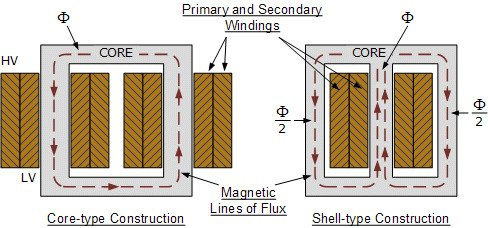
\includegraphics[width=0.6\textwidth]{type_design_2.jpg}
    \caption{Types of three-phase transformers design}
    \label{fig:shell_core_type}
\end{figure}


After a trial and error process using \textit{Gmsh}, the geometries that have been retained is summarized in Table \ref{tab:designed_transfo}. The corresponding transformers with the cotes on it are illustrated on Figures from \ref{fig:Acore} to \ref{fig:Bshell}. 
\begin{longtable}[c]{l|ll|ll}
\caption{Geometry chosen for the two types of core-type three-phase transformers}
\label{tab:designed_transfo}\\

\textbf{Type}                                            & \multicolumn{2}{c|}{\textbf{A}} & \multicolumn{2}{c}{\textbf{B}} \\ \hline
\textbf{Design}                                              & \textbf{Core}     & \textbf{Shell}        & \textbf{Core}       & \textbf{Shell}       \\

\endfirsthead
\multicolumn{5}{c}%
{\tablename\ \thetable\ -- \textit{Continued from previous page}} \\ 
\textbf{Type}                                            & \multicolumn{2}{c|}{\textbf{A}} & \multicolumn{2}{c}{\textbf{B}} \\ \hline
\textbf{Design}                                              & \textbf{Core}     & \textbf{Shell}        & \textbf{Core}       & \textbf{Shell}       \\

\endhead
\multicolumn{5}{r}{\textit{Continued on next page}} \\
\endfoot
\endlastfoot

Height of the window(s) (w\_window) [m]                                             & 3.5 & 3.5  & 4  & 6            \\
Width of the external legs (w\_ext\_leg) [m]                                          & N/A           & 1    & N/A             &  N/A           \\
Width of the intermediary legs (w\_int\_leg) [m]                                      & 1.5         & 1.5  & 3         &   1        \\
Width of the central leg (w\_leg) [m]                                            & 1            & 1    & N/A          & 4            \\
Thickness of the core [m]                                               & 2.2          & 2.2  & 3.35         & 4.75            \\
Cross-section area of the external legs, $S_{external}$ [m$^2$]         & N/A          & 2.2  &  N/A        &  N/A           \\
Cross-section area of the intermediary legs, $S_{intermediary}$ [m$^2$] & 3.3          & 1.5  & 11.5          & 4.75          \\
Cross-section area of the central leg, $S_{central}$ [m$^2$]            & 2.2          & 2.2    & N/A          & 19           \\
Internal transformer ratio, $N_{int}$ [\%]                              & 17.5         & 17.5 & 7            & 7.1          \\
Number of turns - primary, $N_1$ [turns]                                & 400          & 400  & 200          & 450          \\
Number of turns - secondary, $N_2$ [turns]                              & 70           & 70   & 14           & 32           \\
Total height of the transformer [m]                                     & 6.5          & 6.5  & $10\times 3$ & $12\times 3$ \\
Total width of the transformer [m]                                      & 7            & 10   & $10\times 3$ & $12\times 3$        
\end{longtable}
\begin{figure}[h]
    \centering
    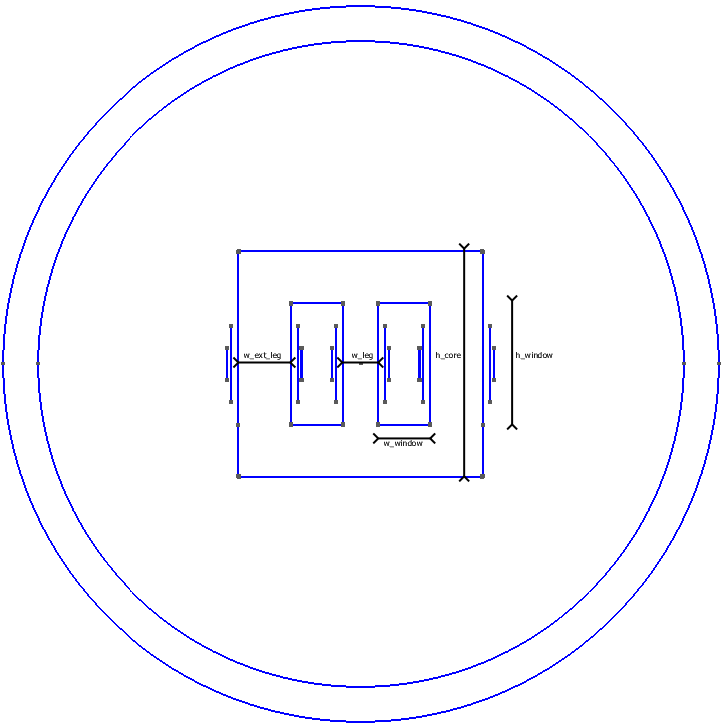
\includegraphics[width=0.5\textwidth]{"Transfo - géometries/transfoA_core.png"}
    \caption{Transfo A - core}
    \label{fig:Acore}
\end{figure}
This first geometry represent the transformer \textbf{A} using the core configuration. As it can be noticed, the retained design is a mono-core where the three phases are magnetically coupled. This allows to produce a compact transformer. 

Here, the three phases does not see the same environment. Indeed, the central winding is trapped in the core while the external windings are partly directly in contact with the surrounding air. This leads to an non symmetry regarding the three phases. Through simulations, an non even distribution of the current between the three phases have been noticed due to this non-symmetry.

On the graph, the long windings are the one corresponding to the primary windings.
\newpage
\begin{figure}[h]
    \centering
    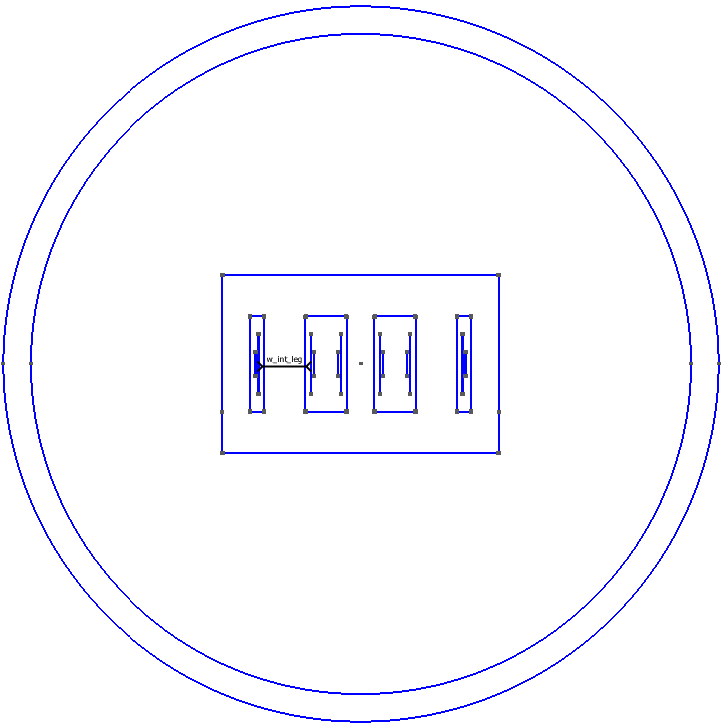
\includegraphics[width=0.5\textwidth]{"Transfo - géometries/transfoA_shell.png"}
    \caption{Transfo A - shell}
    \label{fig:Ashell}
\end{figure}

The second design considered for the low power transformer is the shell design. Here, the "external" coils are surrounded by a magnetic material as well. Thus, the the non-symmetry described earlier disappear using this design.

\begin{figure}[h]
    \centering
    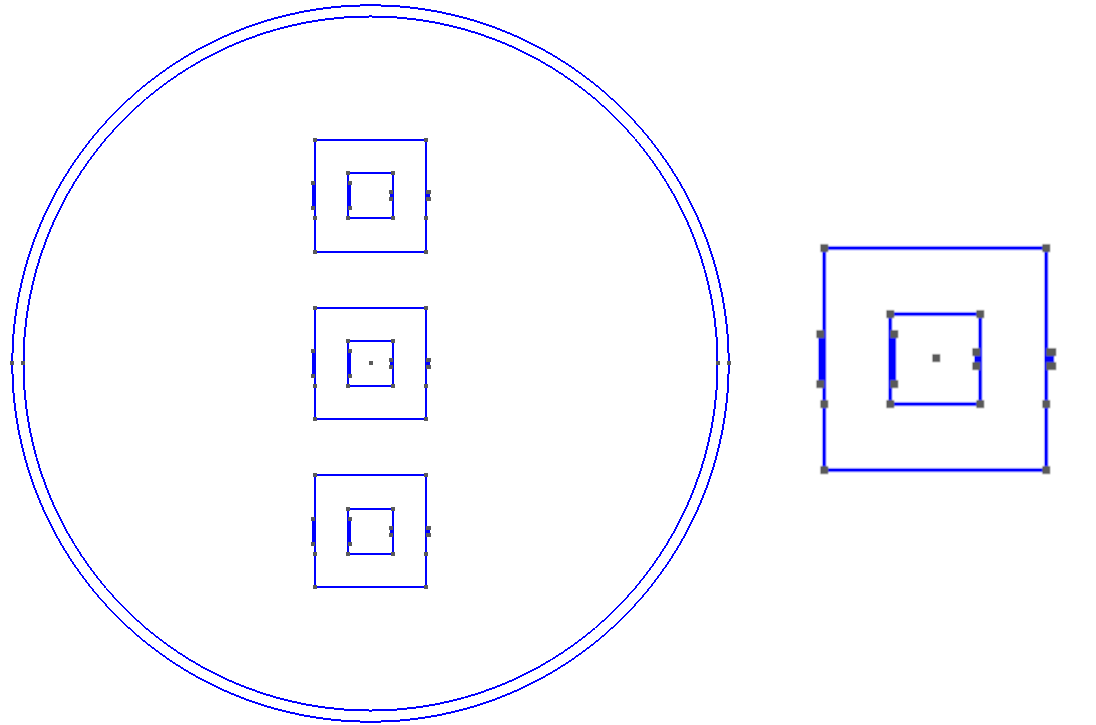
\includegraphics[width=0.65\textwidth]{"Transfo - géometries/transfoB_core.png"}
    \caption{Transfo B - core}
    \label{fig:Bcore}
\end{figure}

Now, considering the high power transformer \textbf{B}, a configuration based on three separated core for each of the phases has been selected. Indeed, the transformer has quite large dimensions. Therefore, separating the three phases allows to ease the installation of the three-phase transformer.

As for the transformer \textbf{A}, the core and shell design have been studied. Figure \ref{fig:Bcore} depicts the chosen design. The magnetic coupling between the three phases is now quasi nonexistent since the surrounding air physically separate each of the three phases.

\begin{figure}[h]
    \centering
    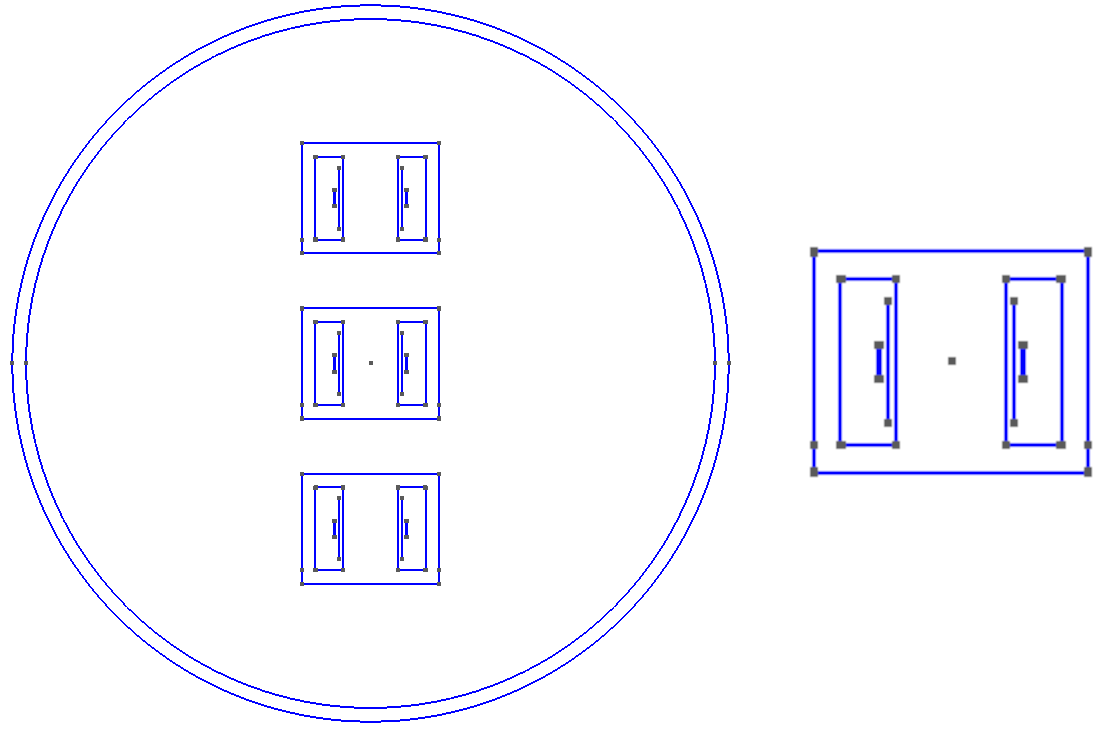
\includegraphics[width=0.65\textwidth]{"Transfo - géometries/transfoB_shell.png"}
    \caption{Transfo B - shell}
    \label{fig:Bshell}
\end{figure}

Finally, Figure \ref{fig:Bshell} shows a picture of the shell design of the transformer \textbf{B}. As for the transformer \textbf{A}, the shells even up the current distribution between the three phases. However, the phenomena is less pronounce than for transformer \textbf{A} since the phases are here not coupled.
\section{Equivalent circuits}
\quad\, This section is dedicated to the determination of the equivalent circuit parameters of the four selected designs. The equivalent circuit is useful to then provide methods to create numeric model of the transformer based on electric circuit. Figure \ref{fig:equivalent_circuit} depicts a generic equivalent circuit.

 \begin{figure}[h]
    \centering
    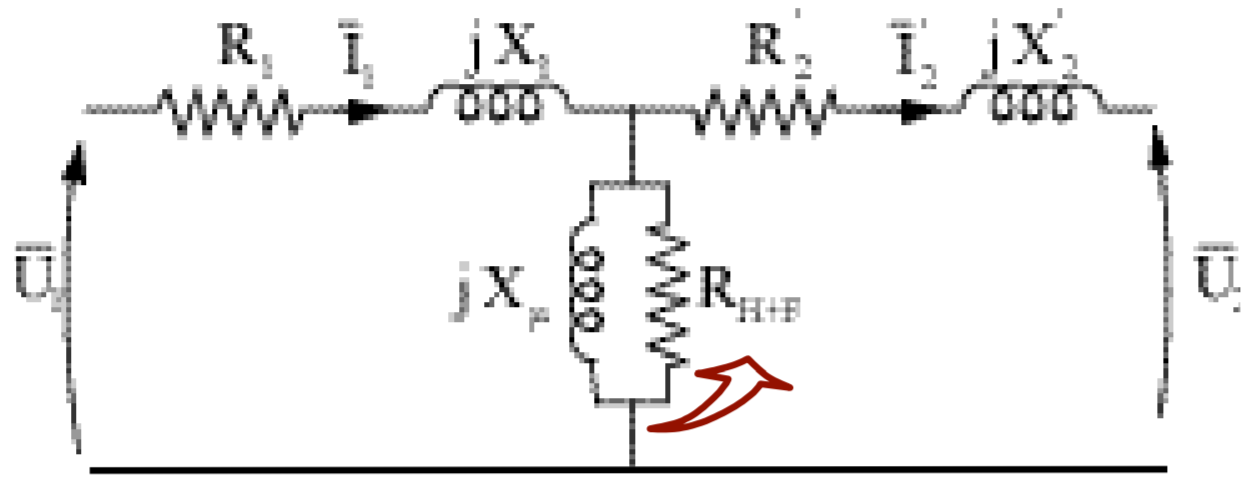
\includegraphics[width=0.6\textwidth]{equivalent_circuit.PNG}
    \caption{Transformer equivalent circuit}
    \label{fig:equivalent_circuit}
\end{figure}

On the diagram, the four parameters R, X, R$_\text{E}$, and X$_\mu$ have to be determined experimentally by performing two different tests, namely the \textbf{open-load} and the \textbf{short-circuit}. 

\subsection{Open-circuit test}
The first test consist in connecting a load of infinite resistance at the terminal of the secondary. Then, the primary side is fed by a voltage source with a set-point fixed at the nominal voltage specified in Table \ref{tab:characteristics_transfo}. 

S 
\subsubsection{Open-load test}
This test is used to calculate the loss in the magnetic circuit (core losses). It is carried out by fixing the resistance of the secondary side to a very high value. In this case, we have $I_1 =$ 7 A and $I_2 =$ 0 A. Using the fact that the electrical power dissipated in $R_1$ and $X_1$ can be neglected, the value of $R_{H+F}$ for the core-type B design can be computed by

\begin{equation}
   P_V = \frac{U_1^2}{R_{H+F}}
\end{equation}

Which leads to

\begin{equation}
    R_{H+F} = \frac{U_1^2}{U_1 \cdot I_1} = \frac{48989,79^2}{48989,79 \cdot 7} = 6998,54 \Omega
\end{equation}
Then the current through $R_{H+F}$ is

\begin{equation}
    I_{R_{H+F}} = \frac{U_1}{R_{H+F}} = \frac{48989,79}{6998,54} = 7 A
\end{equation}
The current through $X_\mu$ can be calculated by 

\begin{equation}
    \|I_{\mu}\| = \sqrt{{I_1}^2 - {I_{R_{H+F}}}^2}
\end{equation}
Then the parameter $X_\mu$ is

\begin{equation}
    X_\mu = \frac{\|U_1\|}{\|I_{\mu}\|} = ... \Omega
\end{equation}

Knowing the imaginary part of the power, this parameter could also be calculated by 
\begin{equation}
   Q_v = \frac{U_1^2}{X_{\mu}}
\end{equation}

\subsubsection{Short-circuit test}
This test is used to determine the copper loss that occurs on the windings at full load. In practice, it is done by fixing the resistance of the secondary side as close to zero as possible. In this case, $I_{cc} = I_1 = 273 A$. The equivalent resistance (in sum) are computed by
\begin{equation}
P_{cc} = (R_1 + R_2') \cdot I_{cc}^2
\end{equation}
Where $I_{cc}$ is the short circuit current (thus maximal nominal current) and has been calculated previously. Then, we have

\begin{equation}
    R_1 + R_2' = \frac{P_{cc}}{{I_1}^2} = \frac{48989,79 \cdot 192,45}{192,45^2} = 246,35 \Omega
\end{equation}
Finally, the sum of leakage reactance are computed by
\begin{equation}
Q_{cc} = (X_1 + X_2') \cdot I_1^2 \iff X_1 + X_2' = \frac{Q_{cc}}{I_1^2}
\end{equation}

Where the reactive power is given by

\begin{equation}
    Q = \sqrt{(U_1 \cdot I_1)^2-P^2} = \sqrt{(U_1 \cdot I_1)^2-P^2} = .. var
\end{equation}

\begin{equation}
    \iff X_1 + X_2' = \frac{Q}{I_1^2} = ... \Omega
\end{equation}

Other values of these parameters for shell-type design have been computed in a similar way and are displayed on Tab.\ref{tab:equivalent_parameters}.

\begin{table}[h]
    \centering
\begin{tabular}{l|ll|ll}
\textbf{Design}                            & \multicolumn{2}{c|}{\textbf{Core}} & \multicolumn{2}{c}{\textbf{Shell}} \\
\textbf{Type}      &     A & B & A & B\\
$R_{H+F}$ [$\Omega$] & & 6998,54 & & \\
$X_\mu$ [$\Omega$] & & & & \\
$R_1 + R_2'$ [$\Omega$] & & 246,35 & & \\
$X_1 + X_2'$ [$\Omega$] & & & & \\
           

\end{tabular}
    \caption{Parameters of the equivalent circuit of the three-phase transformers}
    \label{tab:equivalent_parameters}
\end{table}
%%%%%
% Knowing the value of the losses, the efficiency of the transformers can be calculated using 
% \begin{equation}
%   \eta = \frac{P_{output} [kW]}{P_{input} [kW]}
% \end{equation}
%%%%

\subsubsection{Exterior characteristic}
We can now draw the U-I characteristic for each transformer by varying the charge connected to the secondary side, as shown in the graph below.

\textcolor{red}{Tracer le graphe de $U$ en fonction de $I$ pour les deux types}

\section{Additional parametric studies}

In this section, the influence of a few parameters on the efficiency of the three-phase transformer will be studied.

\subsection{Effect of the winding electric resistivity}
According to Pouillet's law (eq. \ref{eq:pouillet}), we know that increasing the winding electric resistivity will increase the resistance as well and thus decrease the intensity of the currents :

\begin{equation}
    R = \rho \cdot \frac{l}{S}
    \label{eq:pouillet}
\end{equation}
where 
\begin{itemize}
    \item $\rho$ is the electric resistivity of the conductor, which is $2 \cdot 10^{-8} \Omega \cdot m$ for the copper
    \item L its length 
    \item S its cross-section area
\end{itemize}

Efficiency can now be plotted over $\rho$ as a secondary variable, by increasing the electric resistivity (for higher temperatures of the conductor, for example).\\

\textcolor{red}{Tracer le graphe de $\eta$ en fonction de $\rho$}

We can also compute the $I^2R$ component of conductor losses for higher electric resistivity which leads to bigger copper losses.

\subsection{Effect of the core magnetic permeability}
Varying the magnetic permeability has a big impact on the efficiency of the transformer. Indeed, a higher permeability induces a higher efficiency since the field lines are better canalized in the materials, and less losses occur. This figure also confirms that the actual value of magnetic permeability is a good trade-off.

\textcolor{red}{Tracer le graphe de $\eta$ en fonction de $\mu$ + de là, sélectionner un matériau avec un bon $\mu$}

\subsection{Effect of the presence of an air gap}
The presence of air gap increases the total reluctance since the permeability of the air is much smaller than the one of the core because the reluctance of the air is bigger, such as
\begin{equation}
    \Re = \frac{d}{\mu \cdot S} + \frac{e}{\mu_0 \cdot S} \approx \frac{e}{\mu_0 \cdot S}
    \label{eq:total_reluctance}
\end{equation}
with
\begin{itemize}
    \item e the gap space
    \item $\mu_0$ is the magnetic permeability of the air
    \item S the area of the air gap
\end{itemize}

and because 
\begin{equation}
    \mu_{fer} >> \mu_{air} \iff {\Re_{fer}} << {\Re_{air}}
\end{equation}

According to equation \ref{eq:total_reluctance}, an increasing of air gap will increase \textit{e} thus $\Re$ and then the magnetic permeability will decrease, leading to less efficiency.

\textcolor{red}{Tracer le graphe de $\eta$ en fonction de l'air gap (< 0,1 mm)}

\subsection{Effect of a non-laminated core}
There are two main kind of core losses in a transformer : losses by Joule effect due to Eddy current and losses by hysteresis.\\ \\
The Eddy currents are the ones that flow in the core, which is a direct consequence of Lenz's Law. They produce heat, using up energy and then reduce the efficiency of the transformer. In order to get rid of their impact, one possibility is to laminate the core, with laminations separated by thin layers of insulator. In this way, the electrical resistivity in the core increases, leading to less intensities of Eddy currents and thus more efficiency.\\

Without any lamination, the circuiting Eddy current will be enormous through a single mass of the iron core. To simulate the impact of the lack of laminations, the electrical conductivity of the core will be decreased.

\textcolor{red}{Tracer le graphe de $\eta$ en fonction de $\sigma$}

Besides Eddy current, hysteresis losses also generate heat. They are due to reversal of magnetisation in the core (50 times per second for 50 Hz). Hysteresis loss are reduced as much as possible during manufacturing. Note also that both losses can not be zero. Inherent losses will be there, even if the transformer is not connected to any load.\\

Another solution is to use materials which are not conductive, like ferrite.
But this solution will be avoided because it can be very useless at low frequency (as 50 Hz).

\subsection{Effect of shielding the transformer}
Shielding the transformer consists in surrounding it with a high conductivity metal or high permeability material tank in order to reduce the leakage magnetic flux density along the magnetic path.\\

\textcolor{red}{rajouter un volume qui englobe le transfo dans la géométrie + photo}

To see the shielding effectiveness, the leakage magnetic flux density outside the metal tank is compared with the case where there is no tank, so the tank material is considered as the air in this case.

\textcolor{red}{lancer simu + photo before/after the tank}

The shielding effectiveness is evaluated here only by watching the maximal value of B in both cases.


\subsection{Effect of higher operating frequencies}
As said previously, to not exceed the saturation induction of the core, there are minimum values of the number of turns and thus a minimum value of the frequency too, defined by

\begin{equation}
\setstretch{1}
    f > \frac{V_{int}}{2 \cdot \pi \cdot B_{max}\cdot n_1 \cdot S}\label{eq:f_min}
\end{equation}

It also has maximum frequency to minimize the losses. As a remind, losses due to Eddy current are $\propto \omega^2$ and losses by hysteresis are $\propto \omega$. So there is a \textit{frequency range} [$f_{min}$,$f_{max}$] over which the transformer is considered to give satisfactory performances. Beyond this range, the efficiency of the transformer drops.

\textcolor{red}{Tracer le graphe de $\eta$ en fonction de $f$ ou $\omega$}

\subsection{Effect of the loss of one phase}
The loss of a phase means that one phase of the three phases is physically disconnected on the primary side of the transformer. This is often an unintentionally action, so it can simulate a broken conductor that leads to an open phase for example.\\

The effect of the loss of one phase depends on the reasons for choosing a star or delta configuration for transformer winding connections. For example, star connections allows high range of voltages while delta connections are more reliable, meaning that if one winding stop working the other two can still maintain full line voltages to the load.

\section{Conclusion - Limitations - Further work}
Mettre les limites du modèle (cooling methods, insulating oil not discussed here, sélection du type d'enroulement selon la puissance apparente, ..)

\end{document}
